\documentclass[11pt]{article}

\usepackage{hyperref}
\usepackage{enumitem}
\usepackage{epigraph}
\usepackage{comment}
\usepackage{marginnote}
\usepackage{graphicx}
\usepackage[utf8]{inputenc}
\usepackage[english]{babel}
\usepackage[numbers]{natbib}
\usepackage{xspace}
\usepackage{pdflscape}
\usepackage{tabu}

\graphicspath{{img/}}

\setlist[itemize]{itemsep=0mm}

\renewcommand{\familydefault}{\sfdefault}
\renewcommand{\epigraphsize}{\tiny}
\newcommand{\status}[1]{{\texttt{\footnotesize [#1]}}}
\newcommand{\PATHS}{\texttt{PATHS}\xspace}

\title{On the design of AntidoteFS}
\author{Paolo Viotti}
\date{\today}

\begin{document}
\maketitle

\begin{abstract}
This document is a work-in-progress blueprint
for an implementation of an available, distributed POSIX-like file system \cite{posix}
built around the concept of CRDT \cite{crdts-sss}.
Currently, the file system is backed by Antidote \cite{antidote-web},
which exposes an API to interact with CRDTs.
In each section of this document, we elaborate on a different 
way of emulating a file system data model using Antidote 
and its CRDTs library.
\end{abstract}

\begin{comment}
\epigraph{
Alors, plus tard, je l'ai revu Cour de Rome. Alors 
il \'{e}tait avec un copain.  
Alors, il lui disait, le copain : tu devrais faire 
mettre un autre bouton \`{a} ton pardessus. Alors.}
{\textit{Exercices de style, Raymond Queneau}}
\end{comment}

\begin{flushright}
{\footnotesize \ttfamily
\noindent
Antidote v. 0.1.0-git-HEAD\\
%Antidote Java client v. 0.1.0\\
Antidote Javascript client v 0.1.7\\
FUSE v. 2.9.7
}
\end{flushright}
%\vspace{0.5cm}


\section{Directories as maps, files as registers \status{implemented, abandoned}}
\label{sec:design1}
A simple way of emulating a file system data model with Antidote
consists in using its library of CRDTs to model directories as \textit{add-wins maps} %(\texttt{map\_aw})
and files as \textit{last-writer-wins registers}. %(\texttt{lww\_register}).
%
In this way, nesting directories and files inside directories results in
embedding registers and maps inside maps.
Thus, the hierarchical structure of the file system is 
reflected by the actual nesting of CRDT objects.
%
This design has the benefit of being easy to implement and to reason about.
Besides, there is no need to check for cycles, as there cannot be any, since the tree structure is 
enforced in the data model.

Unfortunately, a number of disadvantages and various implementation quirks 
have to be taken into account:
\begin{enumerate}
\item since the hierarchical structure is reflected in the data model, 
when moving files and directories, data has to be moved around across maps and registers in Antidote;
\item there is currently no support for operations on file system metadata (e.g., hard and soft linking, 
permission management, etc), due to lack of metadata attached to CRDTs \status{TODO \cite{antidote-md}};
\item due to the lack of support for nested objects in the Antidote API \cite{antidote-nesting}, 
traversing the file system and writing nested objects is impractical and inefficient;
\item owing to a design choice, in Antidote, object creation and update are not distinguishable.
As a result of this semantics, an attempt to read a non-existing object will return an empty object.
Therefore, to distinguish empty directory from not existing ones, we use \textit{directory markers}, 
i.e. empty registers inside maps;
\item \label{partial-reads} Antidote CRDT maps do not support partial reads or key listing.
Therefore, in order to list the files embedded in a given map, 
one has to read the entire content of a map, and thus, all the data of the objects 
embedded into it. This is clearly not efficient.
\end{enumerate}

Ultimately, due to its overall inflexibility and to the poor support in Antidote 
for nested objects and partial reads, this design has been abandoned.
However, its implementation is still available for future peruse and comparison \cite{antidotefs-nesting}.
Figure~\ref{fig:design1} illustrates the design discussed in this section.

\begin{figure}
	\centering
	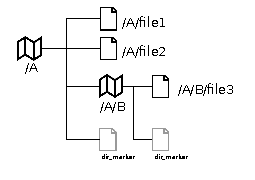
\includegraphics[scale=1.2]{design-1.pdf}
	\caption{Antidote data structures for design option 1. %directory as maps, files as registers.\\
		Antidote's registers and maps are represented 
		respectively with file and map icons.}
	\label{fig:design1}
\end{figure}

%\subsection{Operations}
%\subsubsection{create file}
%\subsubsection{create dir}
%\subsubsection{mv dir }
%\begin{itemize}
%\item copy delete
%\item using a bounded couter as lock
%\end{itemize}


\section{A map of paths, and key indirection \status{implemented, abandoned}}
\label{sec:design2}
To overcome the drawbacks discussed in Sec.~\ref{sec:design1},
in this section, we describe an alternative design that decouples
the file system hierarchical structure from its content.
Its corresponding implementation with Antidote CRDTs is 
represented in Fig.~\ref{fig:design2}.

In this design scheme, a special CRDT map \PATHS stores a 
series of CRDT registers referring to different paths in the file system.
A register in the \PATHS map stores the key within Antidote
of a map containing all data pertaining to that single path, i.e.
all the data related to a given \textit{inode} \cite{posix}.
The keys of maps storing inodes data are composed by a prefix 
(e.g., ``F\_'' for files and ``D\_'' for directories) and by 
an identifier which guarantees their uniqueness without 
requiring coordination (e.g., a UUID \cite{uuid}).
The \PATHS map is cached locally and refreshed periodically
or upon local updates.
Rename and move operations on inodes are carried out by means of transactions 
on the \PATHS map.
Similarly, deleting inodes entails removing their paths, 
while a client-based background task takes care of removing the maps
storing the corresponding data.

\begin{figure}
	\centering
	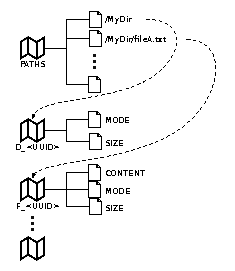
\includegraphics[scale=1.2]{design-2.pdf}
	\caption{Antidote data structures for design option 2. %directory as maps, files as registers.\\
		Antidote's registers and maps are represented 
		respectively with file and map icons.}
	\label{fig:design2}
\end{figure}

While this design is evidently more flexible and better suited to the Antidote data model 
than the one described in Sec.~\ref{sec:design1}, 
it presents some drawbacks.
Namely, as described in Sec.~\ref{sec:design1} (item \ref{partial-reads}), 
read operations on the \PATHS map are total and key listing is not supported.
As a result, refreshing \PATHS map might become onerous as the 
number of paths increases, and listing the files in a directory entails 
scanning the whole keyset of the \PATHS map ($O(n)$).




\section{An inode-based data model \status{80\% implemented}}
\label{sec:design3}
The designs described in the previous sections adopt entities 
like folders, files and paths which are familiar to file systems' users.
As an alternative to this, we propose in this section
a data model which reflects the data model implemented in Unix-like 
file systems and later formalized in the POSIX specification \cite{posix}.
The POSIX standard defines an \textit{inode} data structure
representing file system objects such as files or folders.
The inode data structure, 
which according to POSIX is defined in \texttt{\textless sys/stat.h\textgreater},
includes a number of fields that specify 
ownership, permissions and other metadata of given file system object.

We emulate this basic data structure by using CRDTs as illustrated in Fig.~\ref{fig:design3}.
Each inode is a CRDT map named as \texttt{inode\_X}, where \texttt{X} is the inode number.
The inode map contains a number of LWW registers accounting for permission, 
ownerships and timestamp metadata (e.g., \texttt{ctime}, \texttt{atime}, \texttt{mode}, etc.),
and several other CRDTs that describe the relationships of this inode with 
other inodes.
In particular, if it is a folder inode, it includes a \texttt{children} map that contains 
all references to files and folders names contained in the folder in question.
To each of this name is associated a CRDT add-wins set that contains the inode numbers
of the inode referring to a same name that might be concurrently created at different sites
of the distributed file system.
Conversely, the \texttt{hlinks} CRDT map includes the inode numbers of inode folders that 
contain the file or folder being considered. 
This map and the CRDT integer counter \texttt{nlinks} are updated when performing operations 
like \texttt{unlink}, or when creating hard links of the inode.
In this design, we store the data of a certain inode \texttt{X} in the corresponding 
LWW register called \texttt{data\_X}.

Clearly, this design enjoys the benefits of decoupling the data model 
from the path hierarchy.
However, this translates to an increased difficulty in checking for 
file system structural anomalies such as path cycles.

\begin{figure}
	\centering
	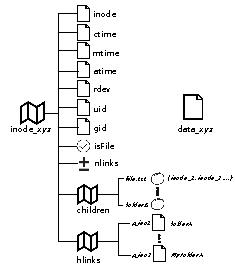
\includegraphics[scale=1.5]{design-3.pdf}
	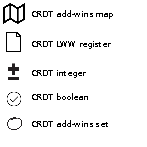
\includegraphics[scale=1.0]{legend.pdf}
	\caption{Antidote data structures for the data model design 
		inspired by the inode data structure.}
	\label{fig:design3}
\end{figure}

\subsection{Conflict management}
A crucial part of designing a distributed file system is 
defining how the POSIX semantics are rendered in a distributed
and fault-prone environment. 
Indeed, a distributed file system will incur a number of
anomalies due to concurrency and faults 
that are not codified by the POSIX standard.
Therefore some conflicts may arise between the file system data 
and metadata seen by different distributed sites.
\citet{Tao.ea:15} classify these conflicts as
\textit{direct} and \textit{indirect} ones. 
Direct conflicts may pertain data, state, mapping or naming,
while indirect conflicts are about the overall structure of the file system
and generally can be seen as a composition of direct conflicts.

%\begin{center}
\begin{table}
	\begin{tabu}to 0.97\textwidth { |X[c] | X[c] | X[c] | X[c]| }
		\hline
		Conflict type & Example & AntidoteFS policy & Notes \\
		\hline
		Naming & Concurrent creation of files and folder with the same name. & Rename files, merge folders. & - \\
		\hline	
		Data & Concurrent updates the same file & LWW or optional lock on file content. & \status{TODO} \\
		\hline	
		State & Concurrent update and delete of a same inode. & Use add-win policy. & - \\
		\hline	
		Mapping  & Divergent concurrent move of folders. & Synchronize move operations. & \status{TODO} \\
		\hline	
		Indirect & Path cycles & Synchronize move operations. & \status{TODO} \\
		\hline		
	\end{tabu}
	\caption{Conflicts types and related resolution policies in AntidoteFS.}
	\label{tab:conflicts}
\end{table}
%\end{center}

%\subsection{Concurrently moving directories \status{TODO}}
%\label{sec:design3-mv}
Table~\ref{tab:conflicts} summarizes the approach of AntidoteFS to these conflicts.
We note that for most concurrent file system operations the 
Antidote's causal+ consistency semantics \cite{rep:pro:sh182} 
is sufficient to preserve the file system invariants and thus avoiding anomalies.
\citet{fs-mahsa} prove that concurrent move operations require
additional coordination.
A coordination mechanism is also needed to avoid editing concurrently a same file.
The implementation of this design scheme \cite{antidotefs}
currently lacks such synchronization mechanism.
A possible way of implementing this would entail exploiting 
bounded counters CRDTs \cite{rep:sh175}
or implementing from scratch a locking primitive in Antidote based
on a total order broadcast implementation.


\section{A tree CRDT \status{TODO}}
\label{sec:design4}
A fourth design option consists in implementing in Antidote a CRDT that would 
enclose the tree-like file system data model and expose an API to
read and update elements of the file systems as they were nodes and edges.

In essence, the data abstraction of a POSIX file system is that of a tree with some additional 
invariants \cite{fs-mahsa}.
Therefore, to implement it as a CRDT one may constrain an existing graph CRDT \cite{crdts-sss}
to comply with both tree and file system invariants \cite{martin:hal-00648106}.

A formal specification of a tree CRDT is currently subject of ongoing work.


\bibliographystyle{plainnat}
\bibliography{predef,refs}

%\clearpage
\appendix

\clearpage
\section{Related work}
In this section we collect a series of related work to study:
\begin{itemize}
\item Git tree objects: \url{https://git-scm.com/book/en/v2/Git-Internals-Git-Objects}
\end{itemize}


\clearpage
%\begin{landscape}
\section{File system, FUSE and Antidote API calls}

\status{TODO}

\begin{center}
\begin{tabular}{c|c|c|c}
	\hline
	CLI commands & FUSE API calls & AntidoteFS logic & Notes \\
	\hline
	\texttt{touch <file>} & - & - & - \\
	\texttt{mkdir <dir>} & - & - & - \\
	\texttt{echo "hello" > <file>} & - & - & - \\
	\texttt{echo "hello" >> <file>} & - & - & - \\
	\texttt{mv <src> <dst>} & - & - & - \\
	\texttt{rm <file>} & - & - & - \\
	
\end{tabular}
\end{center}
%\end{landscape}

\end{document}
